\documentclass{article}
\usepackage{tikz}
\usepackage[utf8]{vietnam}
%%%%%%%%%%%%%%%%%%%%%%%%%%%%%%%%%%%%%%%%%%%%%%%%%%%%%%%
\begin{document}
%%%%%%%%%%%%%%%%%%%%%%%%%%%%%%%%%%%%%%%%%%%%%%%%%%%%%%%

% ! %%%%%%%%%%%%%%%%%%%%%%%%%%%%%%%%%%%%%%%%%%%%%%%%%%%%%%%
\resizebox{0.5\textwidth}{!}{%
% ! %%%%%%%%%%%%%%%%%%%%%%%%%%%%%%%%%%%%%%%%%%%%%%%%%%%%%%%

%%%%%%%%%%%%%%%%%%%%%%%%%%%%%%%%%%%%%%%%%%%%%%%%%%%%%%%
% https://www.mathcha.io/editor
%%%%%%%%%%%%%%%%%%%%%%%%%%%%%%%%%%%%%%%%%%%%%%%%%%%%%%%



\tikzset{every picture/.style={line width=0.75pt}} %set default line width to 0.75pt        

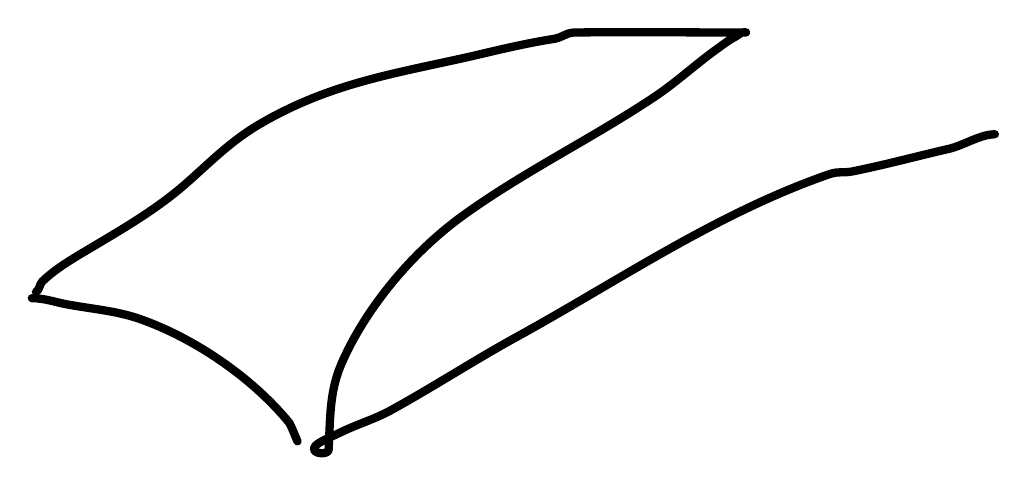
\begin{tikzpicture}[x=0.75pt,y=0.75pt,yscale=-1,xscale=1]
    %uncomment if require: \path (0,300); %set diagram left start at 0, and has height of 300

    %Shape: Free Drawing [id:dp11381719114629973] 
    \draw  [line width=3] [line join = round][line cap = round] (118,183.6) .. controls (124.34,183.6) and (128.93,185.48) .. (135,186.6) .. controls (146.7,188.77) and (158.77,189.67) .. (170,193.6) .. controls (196.33,202.81) and (224.18,221.82) .. (242,243.6) .. controls (242.64,244.38) and (245.83,252.31) .. (246,252.6) ;
    %Shape: Free Drawing [id:dp09156542728828954] 
    \draw  [line width=3] [line join = round][line cap = round] (120,180.6) .. controls (121.74,179.73) and (121.63,176.97) .. (123,175.6) .. controls (127.82,170.78) and (135.09,166.15) .. (141,162.6) .. controls (158.29,152.23) and (176.71,141.98) .. (192,128.6) .. controls (204.07,118.04) and (213.56,108.03) .. (228,99.6) .. controls (263.82,78.71) and (296.66,74.92) .. (336,65.6) .. controls (347.31,62.92) and (358.55,60.36) .. (370,58.6) .. controls (373.13,58.12) and (375.84,55.64) .. (379,55.6) .. controls (406.66,55.27) and (434.33,55.6) .. (462,55.6) .. controls (462.67,55.6) and (460.6,55.3) .. (460,55.6) .. controls (459.06,56.07) and (457.94,57.13) .. (457,57.6) .. controls (453.82,59.19) and (451.31,61.24) .. (448,63.6) .. controls (437.76,70.91) and (428.65,79.5) .. (418,86.6) .. controls (387.74,106.78) and (355.62,122.31) .. (326,143.6) .. controls (299.75,162.47) and (277.86,190.27) .. (267,215.6) .. controls (261.32,228.86) and (261.77,242.04) .. (261,256.6) .. controls (260.88,258.9) and (254.76,258.87) .. (254,256.6) .. controls (253.08,253.85) and (261.61,250.8) .. (266,248.6) .. controls (274.14,244.53) and (283.02,241.99) .. (291,237.6) .. controls (311.1,226.54) and (330.9,213.66) .. (351,202.6) .. controls (401.25,174.96) and (448.37,142.38) .. (503,123.6) .. controls (506.17,122.51) and (509.72,123.26) .. (513,122.6) .. controls (528.78,119.44) and (544.32,115.22) .. (560,111.6) .. controls (566.73,110.05) and (575.13,104.6) .. (582,104.6) ;




\end{tikzpicture}
    
%%%%%%%%%%%%%%%%%%%%%%%%%%%%%%%%%%%%%%%%%%%%%%%%%%%%%%%
% https://www.mathcha.io/editor
%%%%%%%%%%%%%%%%%%%%%%%%%%%%%%%%%%%%%%%%%%%%%%%%%%%%%%%


% ! %%%%%%%%%%%%%%%%%%%%%%%%%%%%%%%%%%%%%%%%%%%%%%%%%%%%%%%
}
% ! %%%%%%%%%%%%%%%%%%%%%%%%%%%%%%%%%%%%%%%%%%%%%%%%%%%%%%%

%%%%%%%%%%%%%%%%%%%%%%%%%%%%%%%%%%%%%%%%%%%%%%%%%%%%%%%
\end{document}
%%%%%%%%%%%%%%%%%%%%%%%%%%%%%%%%%%%%%%%%%%%%%%%%%%%%%%%

